\documentclass[11pt,a4paper]{article}
\usepackage[margin=2.5cm]{geometry}
\usepackage{amsmath}
\usepackage{booktabs}
\usepackage{longtable}
\usepackage{graphicx}
\usepackage[font=small,labelfont=bf]{caption}
\usepackage[hidelinks]{hyperref}
\usepackage{enumitem}
\usepackage{parskip}

\title{\vspace{-1.5cm}What a Tariff That Was Never Collected Cost\\[0.3em]
\large The 2024--26 gold relocation cycle, identified and priced}
\author{Gold flow deconvolution project}
\date{26 August 2026}

\begin{document}
\maketitle

\begin{abstract}
\noindent
Between December 2024 and March 2025, Switzerland sent an estimated 511 tonnes of gold to
the United States over and above what any other Swiss export corridor would predict, and by
July 2026 had taken essentially all of it back. No duty was ever collected on gold. This
memorandum identifies the episode causally and then prices it.

Identification rests on three dated documents that switched US import duty on and off for a
COMEX delivery bar --- executive orders 14257 and 14346 and CBP ruling N351466 --- and on the
fact that the classification hole between them is visible in EO 14346's own annex, where every
gold tariff line except unwrought bullion is flagged as a new addition to the exclusion list.
Five narratively dated events move the COMEX-over-London basis in the predicted direction, with
a joint randomization $p$ of 0.004, while leaving the gold price itself unmoved; a
difference-in-differences against sixteen control corridors puts Switzerland's US corridor first
of seventeen in a placebo distribution whose median is 18 tonnes.

The episode consumed \$243m--\$1,214m in real resources and forgone liquidity services, and
forced \$182m--\$1,977m of revaluation on a hedged short book of 31 million ounces. Gross
bilateral flow was 1,381 tonnes; the net position change was $-1.5$ tonnes. Separately, the
formula that set Switzerland's reciprocal tariff rate is shown to be three times more sensitive
to which year's data goes into it with gold left in than with gold taken out: the same formula
yields 30\% on 2024 data and the 10\% floor on 2026 data, entirely because of which way the
bullion happened to be pointing.
\end{abstract}

\tableofcontents

%==============================================================================
\section{The claim, and what would falsify it}
%==============================================================================

The 2024--26 gold episode is usually told as a story about a tariff. It is better told as a
story about a \emph{classification}, and better still as a demonstration that a policy which is
never implemented is not therefore free.

Three things have to hold for that story to be worth telling.

\begin{enumerate}[leftmargin=*]
\item \textbf{The mechanism has to be real and datable.} If the ``tariff threat on gold'' is
folk narrative rather than a specific legal exposure on specific dates, there is nothing to
identify. \S\ref{sec:mechanism} shows the exposure existed, names the document that created it,
and names the document that closed it.

\item \textbf{The market has to have responded to those dates, and to have responded in the
price of \emph{location} rather than the price of gold.} If the events moved gold generally,
this is a macro story and the relocation is incidental. \S\ref{sec:events} tests both.

\item \textbf{The metal has to have moved because of it.} Swiss--US gold flow was also enormous
in 2020, for reasons that had nothing to do with trade policy. A counterfactual is required, not
a level. \S\ref{sec:flow} builds one and subjects it to a placebo distribution.
\end{enumerate}

Only then does \S\ref{sec:ledger} price it. The pricing is deliberately conservative in one
respect and deliberately generous in another, and the memorandum is explicit about which is
which.

\subsection{What is new here relative to the project's earlier memorandum}

The project's previous memorandum on this episode established the round trip descriptively and
documented the classification anomaly. Four things are added or corrected:

\begin{itemize}[leftmargin=*]
\item \textbf{The third event is now pinned to a document.} The earlier memorandum recorded the
August 2025 resolution as ``not pinned to a document.'' It is: Executive Order 14346 of
5 September 2025. \S\ref{sec:mechanism} shows the hole and its closure inside the order's own
annex.
\item \textbf{The response is identified rather than described.} Event-study and
difference-in-differences estimates with randomization inference replace correlations.
\item \textbf{The band-of-inaction estimate of transfer cost fails, and is reported as
failing.} \S\ref{sec:whatfailed}. The project's earlier finding that ``the threshold is near
zero'' is a weak-identification artefact, not a result.
\item \textbf{The intuition that phantom gold inflated Switzerland's tariff rate is wrong in
sign.} On the 2024 vintage it lowered it. The real problem is variance, not level.
\S\ref{sec:contamination}.
\end{itemize}

%==============================================================================
\section{The mechanism: a hole between two tariff lines}
\label{sec:mechanism}
%==============================================================================

A COMEX gold contract is satisfied by delivering a 100 oz or 1 kg bar of at least 995 fineness
from an approved refiner, stamped with weight, purity and a serial number. The question that
drove this entire episode is which line of the US tariff schedule that object falls under.

\subsection{Three documents}

\textbf{2 April 2025 --- Executive Order 14257.} The reciprocal tariff order carried an
Annex~II of excluded products. Gold appears in it as \texttt{7108.12.10}, ``gold, nonmonetary,
bullion and dor\'e'' --- \emph{unwrought} gold. Everyone read this as ``gold is exempt.'' The
basis collapsed accordingly.

\textbf{31 July 2025 --- CBP ruling N351466.} A Swiss refiner asked Customs and Border
Protection to confirm that PAMP-branded kilo and 100 oz bars were \texttt{7108.12.10}. CBP said
no. Additional US Note 1(a) to Chapter 71 excludes from ``unwrought'' any cast form ``which
[has] been machined or processed otherwise than by simple trimming, scalping or descaling.'' A
bar that has been stamped and laser-marked has been further processed. The bars were classified
under \texttt{7108.13.5500} --- and under \texttt{9903.01.25}, the Chapter 99 provision through
which the reciprocal duties are administered. The standard COMEX delivery bar had become
dutiable without any change in tariff policy at all.

\textbf{5 September 2025 --- Executive Order 14346.} A replacement Annex~II to EO 14257.

\subsection{The hole is visible in the order's own annex}

EO 14346's Annex~II marks each entry that is newly excluded with the word ``Addition.'' Pulling
the Federal Register PDF and reading the flags gives Table~\ref{tab:annex}.

\begin{table}[h]
\centering
\begin{tabular}{@{}llc@{}}
\toprule
\textbf{HTSUS} & \textbf{Description} & \textbf{Flagged ``Addition''} \\
\midrule
7106.91.10 & Silver bullion and dor\'e & no \\
7108.11.00 & Gold, nonmonetary, powder & \textbf{yes} \\
\textbf{7108.12.10} & \textbf{Gold, nonmonetary, bullion and dor\'e} & \textbf{no} \\
7108.12.50 & Gold, nonmonetary, other unwrought forms & \textbf{yes} \\
7108.13.10 & Gold leaf & \textbf{yes} \\
\textbf{7108.13.55} & \textbf{Rectangular shapes, $\geq$99.5\%, marked only with weight/purity} & \textbf{yes} \\
7108.13.70 & Gold, other semimanufactured forms, other & \textbf{yes} \\
7108.20.00 & Gold, monetary & \textbf{yes} \\
\bottomrule
\end{tabular}
\caption{Gold and silver lines in the replacement Annex~II attached to EO 14346, with the
order's own ``Addition'' flag. Retrieved and parsed from the Federal Register PDF for FR
2025-17507, 90 FR 43743, by \texttt{code/01\_events\_and\_us\_che\_trade.py}.}
\label{tab:annex}
\end{table}

The contrast is the whole story. \texttt{7108.12.10} carries no flag because EO 14257's original
Annex~II already excluded it in April. \texttt{7108.13.55} --- the exact line CBP put the COMEX
delivery bar into on 31 July --- \emph{is} flagged. It was therefore not on the exclusion list
between 2 April and 8 September 2025, which is precisely the exposure the market discovered on
8 August.

EO 14346 also inserted the same codes into subdivision (v)(iii) of U.S. note 2 to subchapter III
of chapter 99, removing them from the duty mechanism itself, and section 2(a) made the
replacement annex effective at 12:01 a.m.\ EDT three days after the order --- 8 September 2025.

The reason the earlier memorandum could not pin this is worth recording: the Federal Register's
full-text search does not index the annexes. Querying its API for ``7108'' across August 2025 to
March 2026 returns one document, about social security representative fees. The evidence is in
the PDF appendix, not the searchable text.

\subsection{The market chronology}

Two of the four market-relevant dates are not the document dates. CBP's ruling is dated 31 July
but reached the market on Friday 8 August, when it was reported and gold futures set a record
intraday. The reversal came on Monday 11 August, in a presidential statement --- ``Gold will not
be Tariffed!'' --- that has no Federal Register instrument at all and is dated here from
contemporaneous reporting. EO 14346 followed on 5 September and made the reversal law.

\begin{table}[h]
\centering
\small
\begin{tabular}{@{}lllc@{}}
\toprule
\textbf{Market date} & \textbf{Event} & \textbf{Instrument} & \textbf{Duty risk} \\
\midrule
5 Nov 2024 & US presidential election & --- & rises \\
2 Apr 2025 & Annex II excludes unwrought gold only & EO 14257 / FR 2025-06063 & off (partly) \\
8 Aug 2025 & CBP ruling reaches the market & CBP CROSS N351466 & \textbf{on} \\
11 Aug 2025 & ``Gold will not be Tariffed'' & no instrument & off \\
5 Sep 2025 & Replacement Annex II signed & EO 14346 / FR 2025-17507 & off (in law) \\
\bottomrule
\end{tabular}
\caption{Event chronology. Document identifiers retrieved from the Federal Register and CBP
CROSS APIs.}
\end{table}

%==============================================================================
\section{The price of location responded, the price of gold did not}
\label{sec:events}
%==============================================================================

\subsection{Outcome and inference}

The outcome is the \emph{excess basis}: the COMEX settlement price minus the LBMA PM auction
price, minus the carry the delivery calendar mechanically implies. Working in dollars per ounce
net of carry rather than in the raw spread matters because \texttt{GC1} rolls through six
delivery months a year and the raw spread carries a sawtooth of tens of dollars driven purely by
time to delivery. Net of that, the excess basis is what an arbitrageur is paid for having metal
in New York rather than London.

Each event is anchored at the last COMEX settlement that could not contain the news --- gold
settles at 13:30 ET, so an announcement at 16:00 belongs to the next session --- and the response
is measured forward. The sign expected of each event was fixed by the direction of the policy
change before the series was examined.

Inference is by randomization. The null is the empirical distribution of the same statistic
computed at every non-event date from 2015 to 2026, with a ten-observation buffer around each
event removed. Nothing is assumed about its shape, which matters because the basis is
fat-tailed.

\subsection{The measurement problem, and why it makes the test conservative}

The COMEX leg settles at 13:30 ET; the London leg is the 15:00 London PM auction, three and a
half hours earlier. The excess basis therefore carries a non-synchronous-pricing error whose
daily standard deviation is about \$16 per ounce --- close to gold's own daily volatility. That
error is in the outcome, not in the treatment. It inflates the randomization null and makes
every test below harder to pass, not easier. It also, as \S\ref{sec:whatfailed} shows, destroys
a different estimator entirely.

\subsection{Results}

\begin{table}[h]
\centering
\small
\begin{tabular}{@{}lrrrrrr@{}}
\toprule
& \multicolumn{3}{c}{\textbf{Excess basis (USD/oz)}} & \multicolumn{3}{c}{\textbf{Gold price (placebo)}} \\
\cmidrule(lr){2-4}\cmidrule(lr){5-7}
\textbf{Event} & \textbf{move} & \textbf{$z$} & \textbf{$p$} & \textbf{move} & \textbf{$z$} & \textbf{$p$} \\
\midrule
Election, 5 Nov 24 \hfill \emph{1-day}       & $+9.6$  & $+0.60$ & 0.157 & $-2.29$ & $-3.01$ & \textbf{0.012} \\
EO 14257 Annex II, 2 Apr 25 \hfill \emph{3-day} & $-48.2$ & $-4.40$ & \textbf{0.003} & $-1.96$ & $-1.43$ & 0.138 \\
CBP N351466 reported, 8 Aug 25 \hfill \emph{1-day} & $+27.5$ & $+1.70$ & \textbf{0.028} & $+0.31$ & $+0.30$ & 0.667 \\
``Gold will not be Tariffed'', 11 Aug 25 \hfill \emph{1-day} & $-46.9$ & $-2.91$ & \textbf{0.010} & $-0.85$ & $-1.10$ & 0.201 \\
EO 14346 signed, 5 Sep 25 \hfill \emph{3-day} & $-28.4$ & $-2.59$ & \textbf{0.012} & $+2.18$ & $+1.59$ & 0.109 \\
\midrule
\multicolumn{7}{@{}l@{}}{\emph{Joint test, sum of sign-adjusted one-day moves: $+\$139.4$/oz, randomization $p = 0.0039$}} \\
\bottomrule
\end{tabular}
\caption{Event study. The excess-basis $p$-values are one-sided in the predicted direction; the
gold-price $p$-values are two-sided, since no direction was predicted for the placebo. $z$ is
against each series' own randomization null ($n=2{,}330$ non-event windows for the one-day
statistic). Both the one-day and three-day windows are computed for every event; the row shows
the window with the smaller $p$ and the other is written to
\texttt{output/event\_study\_windows.csv} by the script. The three-day statistic is the mean over the three
observations after the anchor less the mean over the three ending at it.}
\label{tab:events}
\end{table}

Three readings.

\textbf{The four gold-specific policy events moved the price of location, and none moved the
price of gold.} All four clear conventional significance on the basis; none does on spot. The
joint test, which fixes each sign in advance and resamples five one-day moves from non-event
days, gives $p = 0.0039$.

\textbf{The election is the mirror image, and that is the cleanest falsification test in the
memorandum.} It moved gold by three standard deviations ($p = 0.012$) and the location premium
not at all. If these tests were picking up general market turbulence, the largest macro event in
the sample would show up in the basis. It does not. The election repriced gold; the
classification rulings repriced its address.

\textbf{The August pair is a two-session on/off switch.} The excess basis rose \$27.48 on
8 August, to a raw COMEX-over-London spread of \$97.15 --- and fell \$46.95 on 11 August. Over
those same two sessions the gold price moved $+0.31\%$ and $-1.11\%$. A rumour and its denial,
two business days apart, moved the cost of having metal in the wrong city by more than seventy
dollars an ounce.

\begin{figure}[htbp]
\centering
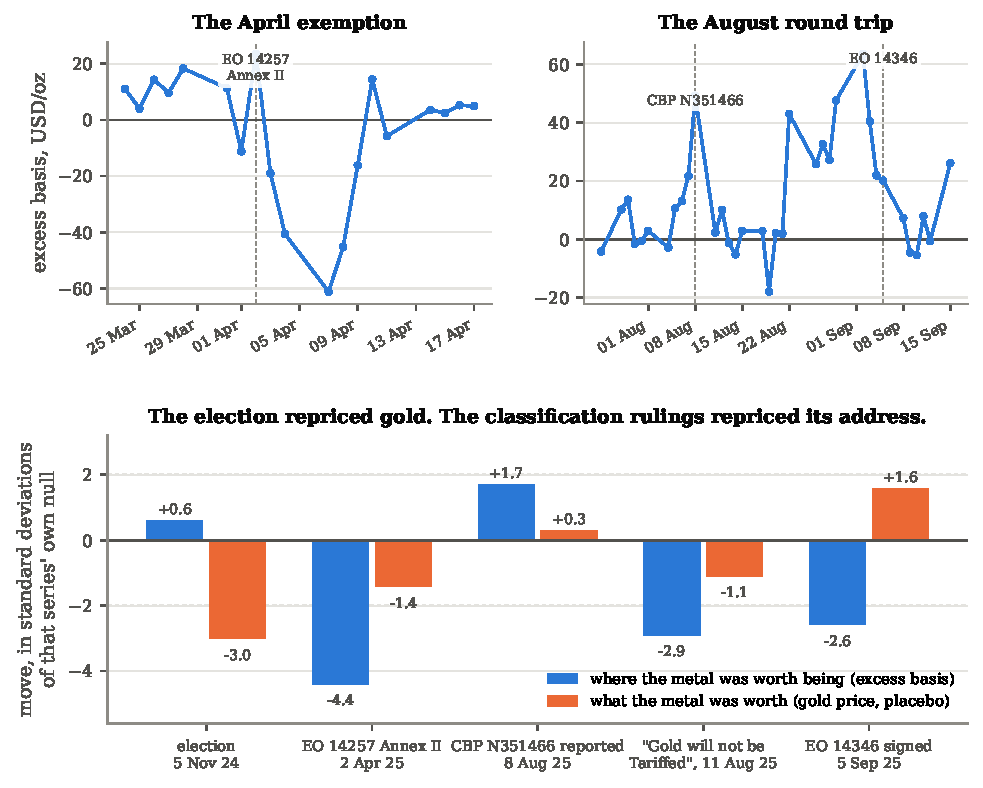
\includegraphics[width=\textwidth]{figures/fig2_event_study.pdf}
\caption{Top: the excess basis through the two windows in which policy landed, with event dates
marked. Bottom: each event's move in standard deviations of its own randomization null, for the
location premium and for the gold price.}
\end{figure}

%==============================================================================
\section{How much metal the threat moved}
\label{sec:flow}
%==============================================================================

\subsection{Design}

Switzerland's gold exports are a panel: one series per destination, monthly, in tonnes, from
BAZG's bulk customs files. The United States is the treated corridor. Sixteen other destinations
that traded in at least 80\% of pre-treatment months and averaged at least 0.2 t/month form the
control group.\footnote{AE, AT, CN, DE, FR, GB, HK, IN, IT, KR, LB, MY, SG, TH, TR, TW. The
admission rule is deliberately loose: the placebo $p$-value cannot fall below
$1/(\text{donors}+1)$, so a thin pool caps inference before the data does.} A two-way
fixed-effects event study with October 2024 as the omitted month gives the tonnes per month by
which the US corridor departed from what its own average level and the month's common shock
predict.

Inference is an in-space placebo: the entire estimation is re-run pretending each control
corridor was treated.

\subsection{Results}

\begin{table}[h]
\centering
\small
\begin{tabular}{@{}lrrrrr@{}}
\toprule
\textbf{Corridor and window} & \textbf{DiD (t)} & \textbf{t/month} & \textbf{Treated-only (t)} & \textbf{Placebo rank} & \textbf{$p$} \\
\midrule
CHE $\to$ US, Dec 24 -- Mar 25 & \textbf{510.7} & 127.7 & 495.5 & \textbf{1 of 17} & \textbf{0.059} \\
CHE $\to$ US, Apr 25 -- Jul 26 & $-28.8$ & $-1.8$ & $-28.0$ & 9 of 17 & 0.529 \\
US $\to$ CHE, Dec 24 -- Mar 25 & $-0.5$ & $-0.1$ & $-2.2$ & 40 of 41 & 0.976 \\
US $\to$ CHE, Apr 25 -- Jul 26 & \textbf{348.4} & 21.8 & 322.3 & 3 of 41 & 0.073 \\
\bottomrule
\end{tabular}
\caption{Difference-in-differences on Swiss gold trade with the United States. ``Treated-only''
is the same excess measured against the corridor's own 2015--2024 mean, ignoring the controls
entirely. Placebo rank is the position of the treated effect in the distribution of absolute
effects when each control corridor is treated in turn.}
\label{tab:did}
\end{table}

The westbound surge is 510.7 tonnes over four months, and it is first of seventeen. The median
absolute placebo effect over the same window is 18.4 tonnes and the largest is 97.9 tonnes; the
treated effect is 5.2 times the largest placebo and 28 times the median. The $p$-value of 0.059
is the floor with sixteen donors, not a weak result --- no control corridor comes close.

The design's own internal placebo is the third row. If this were a general Swiss--US shipping
shock, or a data artefact in the corridor, the eastbound leg would move during the surge too. It
ranks 40th of 41. The return leg then appears in the fourth row, in the window where the
mechanism says it should be, and nowhere else.

Pre-trends are flat. Over the eighteen months before October 2024 the mean absolute event-time
coefficient is 6.4 tonnes per month, against a surge effect of 127.7 --- twenty times larger.

\begin{figure}[htbp]
\centering
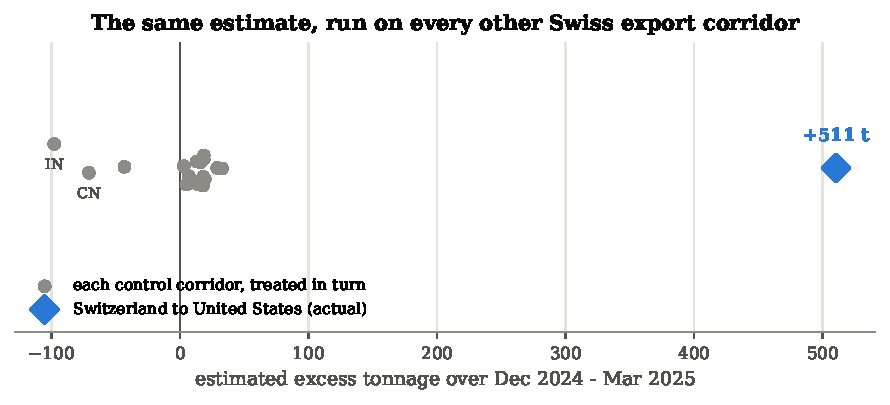
\includegraphics[width=\textwidth]{figures/fig4_placebo.pdf}
\caption{The in-space placebo distribution. Each grey point is the same estimate run on one
control corridor.}
\end{figure}

\subsection{The assumption that fails, and what it costs}

No-interference between corridors does not hold, and pretending otherwise would be dishonest.
Swiss refining and secure-logistics capacity is finite over a few months. During the surge:

\begin{center}
\small
\begin{tabular}{@{}lr@{}}
\toprule
Total Swiss gold exports, pre-treatment mean & 137.5 t/month \\
Total Swiss gold exports, Dec 2024 -- Mar 2025 & 190.8 t/month \\
\midrule
US corridor & $+123.9$ t/month \\
All control corridors & $-70.8$ t/month \\
\emph{of which} India & $-25.0$ \\
\emph{of which} China & $-23.6$ \\
\emph{of which} Hong Kong & $-13.2$ \\
\bottomrule
\end{tabular}
\end{center}

Fifty-seven per cent of the rise in the US corridor was offset by falls elsewhere. Swiss output
was redirected as much as expanded. This biases the difference-in-differences upward, because
the control corridors' fall lowers the common time effect --- which is why Table~\ref{tab:did}
also reports the treated-only estimate, 495.5 tonnes, that ignores the controls. The two bound
the answer at roughly 496--511 tonnes, a 3\% spread, so the headline is not sensitive to which
one is preferred.

The displacement is not merely a nuisance. Roughly 283 tonnes of gold that would have gone to
India, China and Hong Kong over four months went to a vault in New York instead. Consumption
markets short of metal pay a premium for it, and that premium is a transfer from households in
Asia to whoever supplied them. \S\ref{sec:ledger} reports the tonnage and declines to price it,
because pricing it needs local premium series this project has not pulled.

\begin{figure}[htbp]
\centering
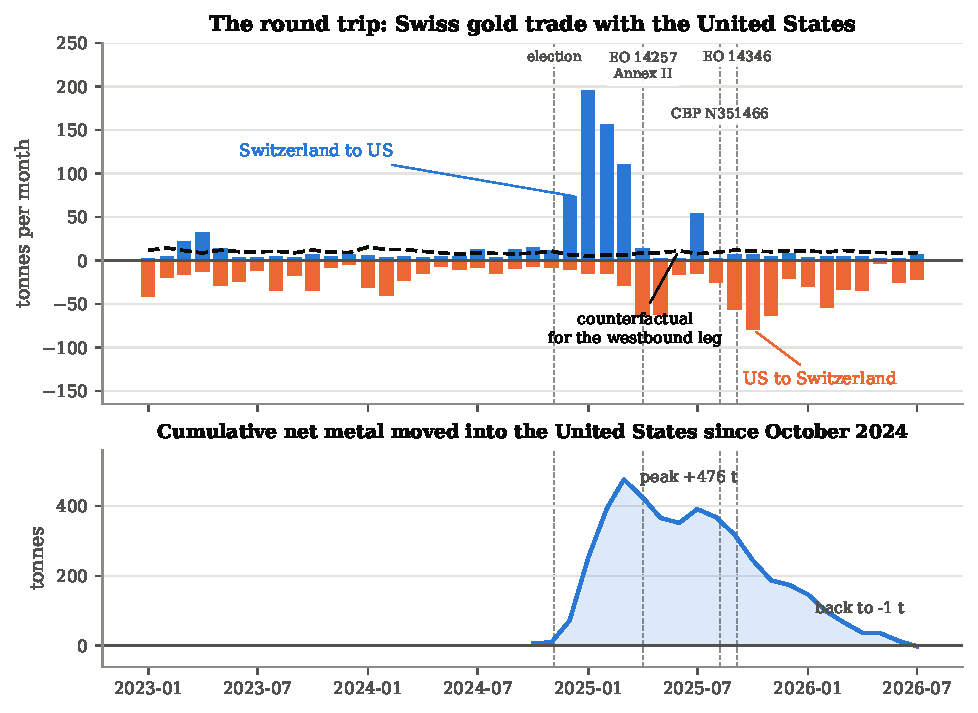
\includegraphics[width=\textwidth]{figures/fig1_relocation_cycle.pdf}
\caption{The relocation cycle. The dashed line is the difference-in-differences counterfactual
for the westbound leg. Cumulative net metal peaks at $+476$ tonnes and returns to $-1$ tonne.}
\end{figure}

%==============================================================================
\section{The same shock, twice, with the escape route open and then closed}
\label{sec:regimes}
%==============================================================================

The episode ran the same experiment twice under different conditions, and the contrast is the
central economic result of this memorandum.

\begin{center}
\small
\begin{tabular}{@{}lrrr@{}}
\toprule
& \textbf{Trading days} & \textbf{Mean excess basis} & \textbf{Excess tonnes} \\
\midrule
Calm baseline, 2015--2019 & 1,038 & \$0.07 & --- \\
Dec 2024 -- Mar 2025, arbitrage executable & 63 & \$5.44 & \textbf{511} \\
8 Aug -- 8 Sep 2025, arbitrage blocked & 20 & \textbf{\$18.82} & \textbf{0} \\
\bottomrule
\end{tabular}
\end{center}

In the first window the duty was not in force and there were five months of runway. A dealer
short COMEX against London metal could ship. Quantity adjusted, and the price stayed close to
the cost of shipping: a mean excess basis of \$5.44 an ounce, on a \$2,800 metal, while half a
thousand tonnes crossed the Atlantic.

In the second window the duty was already attached to the delivery bar by CBP's ruling. Shipping
metal in would have meant paying it on arrival. Quantity could not adjust, so the price took the
entire shock: a mean excess basis three and a half times larger, a peak of \$63.60 over carry and
\$102.20 in raw spread --- the widest of the whole era --- and almost no metal moved.

This is the textbook consequence of a kinked arbitrage constraint, and it has a direct bearing
on how the episode should be costed. When arbitrage is open, the cost of a policy threat shows
up as \emph{quantity}: real resources burned moving metal that did not need moving. When
arbitrage is closed, it shows up as \emph{price}: transfers from whoever is on the wrong side of
a spread they cannot escape. The two are different kinds of cost and \S\ref{sec:ledger} keeps
them in different tiers.

It also answers the question the project's earlier memorandum posed and could not resolve --- why
the widest basis of the era coincided with almost no flow, and why the tariff episode moved so
much more metal per unit of dislocation than COVID-2020 did. The dislocation is not a measure of
how badly metal wanted to move. It is a measure of how badly metal wanted to move \emph{and
could not}.

\begin{figure}[htbp]
\centering
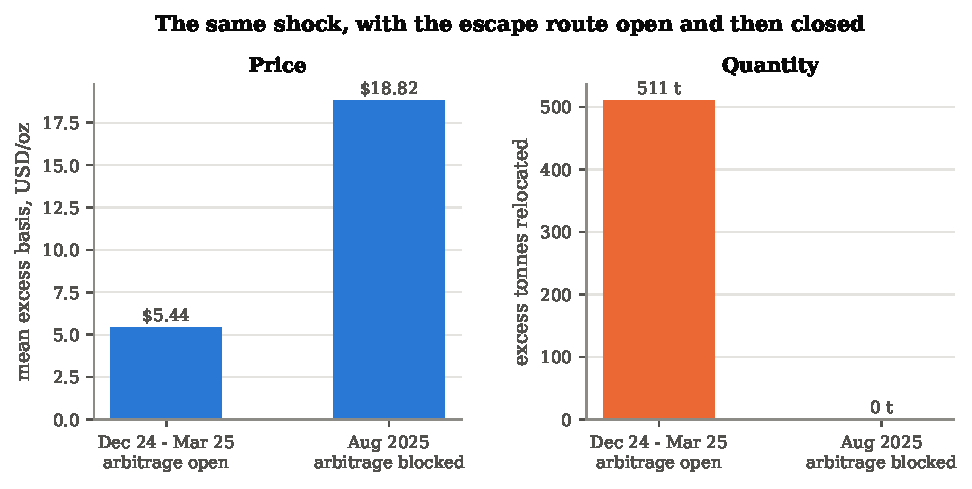
\includegraphics[width=\textwidth]{figures/fig3_price_or_quantity.pdf}
\caption{The same shock under two regimes. Never plotted on shared axes: the point is that one
adjusts when the other cannot.}
\end{figure}

%==============================================================================
\section{The ledger}
\label{sec:ledger}
%==============================================================================

Nobody paid a gold tariff. The question is what the threat cost anyway.

Three kinds of cost are kept apart, because conflating them is how numbers like this get
inflated past the point of usefulness.

\begin{description}[leftmargin=1.2cm,style=nextline]
\item[Tier I --- real resources.] Aircraft, armoured transport, insurance underwriting, refinery
furnace time, assay labour. Burned. The world is poorer by this amount and nobody is richer.
\item[Tier II --- transfers.] The excess basis is paid by one party to another. Not a resource
loss to the system, but a very real loss to whoever is on the wrong side, and the mechanism by
which a policy rumour becomes a margin call.
\item[Tier III --- opportunity cost.] Metal under a COMEX warrant is metal not in the London
lending pool. A real efficiency loss, but not cash out of anyone's pocket.
\end{description}

\subsection{Tier I: moving the metal}

The quantity is measured: 496--511 tonnes westbound plus 322--348 tonnes eastbound, from
\S\ref{sec:flow}. Both legs are charged the full unit cost including recasting, because a round
trip destroys and recreates bar form twice --- London Good Delivery 400 oz bars into
COMEX-deliverable kilobars going out, and back again coming home.

The unit cost is \emph{not} measured, and this is the weakest link in the memorandum.
\S\ref{sec:whatfailed} explains why the attempt to estimate it from market behaviour failed. The
ledger therefore uses a stated bottom-up range and carries the sensitivity through to the
headline:

\begin{center}
\small
\begin{tabular}{@{}lrr@{}}
\toprule
\textbf{Component, one way} & \textbf{Low} & \textbf{High} \\
\midrule
Recasting 400 oz to kilobar or 100 oz & \$0.50 & \$2.00 \\
Secure transatlantic air freight & \$0.30 & \$1.00 \\
Insurance in transit & \$0.10 & \$0.50 \\
Handling, assay, vault in and out & \$0.20 & \$0.80 \\
\midrule
\textbf{Real resources} & \textbf{\$1.10} & \textbf{\$4.30} \\
Forgone lease income in transit (10--20 days) & \$0.51 & \$6.06 \\
\textbf{All in} & \textbf{\$1.60} & \textbf{\$10.36} \\
\bottomrule
\end{tabular}
\end{center}

Only the financing line is derived, from the mean spot price over the episode and an assumed
lease-rate range of 0.5\% to 3\%. The rest are order-of-magnitude assumptions; no public series
for bullion logistics or refining fees exists. Note that transit financing is charged at the
gold lease rate rather than at a short rate: the owner was paying to carry the metal in a London
vault anyway, and shipping it does not add a full SOFR. Charging SOFR, as an earlier draft of the
script did, roughly triples this line and attributes to the episode a cost that would have been
borne regardless.

Gold is extraordinarily cheap to move relative to its value --- a kilobar at \$3,900 an ounce is
a \$125,000 object weighing one kilogram --- and the resulting figure is smaller than intuition
suggests: \textbf{\$29m--\$119m} in real resources, \textbf{\$42m--\$286m} all in.

\subsection{Tier II: the cost of not being able to move}

This is the ``it is not free to drop your short'' line, and the exposed population is measured
rather than assumed. The CFTC's disaggregated Commitments of Traders report gives the short
positions of producers, merchants, processors and users plus swap dealers --- the bucket in which
dealer shorts hedged against unallocated London metal sit. Through the episode that book ran at
31--33 million ounces, about two-thirds of total open interest.

\begin{center}
\small
\begin{tabular}{@{}lrrr@{}}
\toprule
& \textbf{Hedged short book} & \textbf{Excess basis} & \textbf{Revaluation} \\
\midrule
Dec 2024 -- Mar 2025, mean & 33.5 Moz & \$5.44 & \$182m \\
Dec 2024 -- Mar 2025, at peak & 33.5 Moz & \$36.83 & \$1,232m \\
8 Aug -- 8 Sep 2025, mean & 31.1 Moz & \$18.82 & \$585m \\
8 Aug -- 8 Sep 2025, at peak & 31.1 Moz & \$63.60 & \textbf{\$1,977m} \\
\bottomrule
\end{tabular}
\end{center}

Two caveats bound this from above. The CFTC does not report how much of the hedger bucket is
spread against London specifically, so this is the revaluation of the whole hedged short book.
And it is a mark-to-market: only positions actually closed at dislocated levels realised it. What
it does establish is the scale of the pressure. A rumour about a customs classification put a
number close to two billion dollars of adverse revaluation onto a book that had, three sessions
earlier, been flat.

Seen from the other side of the same trade, the parties who shipped the 511 tonnes earned the
basis on it: \$87m--\$89m at the surge window's mean. That is the small number, and it is small
for the reason \S\ref{sec:regimes} gives --- when the arbitrage works, competition drives the
price back down to the cost of doing it.

\subsection{Tier III: metal that stopped working}

COMEX depository stock rose from 974 tonnes on 30 January 2025 to a peak of 1,398 tonnes on
7 April, and drained back to 830 tonnes by August 2026. Integrating the excess over the 30
January level across the whole window gives \textbf{226 registered tonne-years} of metal held
under warrant that would not otherwise have been --- roughly \$28.5bn of metal-years at the
window's mean spot price of \$3,922.

Priced at the gold lease rate plus storage, that is \textbf{\$214m--\$928m} of forgone liquidity
service. The registered figure is used rather than the total because eligible metal, though in
the same warehouse, is not committed to delivery and can still be lent.

This is the most uncertain line in the ledger in one direction and the most conservative in
another. Uncertain, because no free public gold lease-rate series exists and the range spans a
factor of six. Conservative, because the baseline is 30 January 2025, by which date a large part
of the build had already happened: the CME depository reports were recovered from Internet
Archive snapshots, and no snapshot exists between 20 April 2023 and 30 January 2025.

\begin{figure}[htbp]
\centering
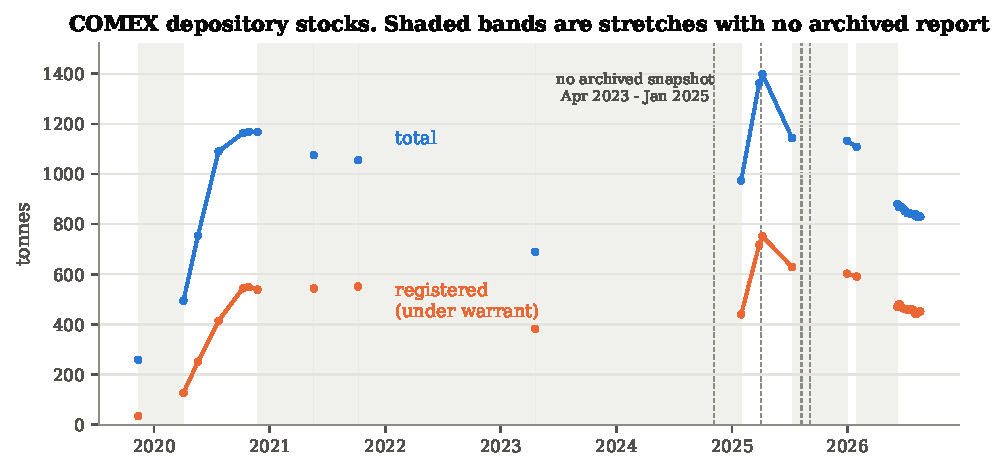
\includegraphics[width=\textwidth]{figures/fig7_comex.pdf}
\caption{COMEX depository stocks. Every observation is a marker; shaded bands are stretches with
no archived report, and are not bridged.}
\end{figure}

\subsection{The total}

\begin{table}[h]
\centering
\begin{tabular}{@{}llrr@{}}
\toprule
\textbf{Tier} & \textbf{Item} & \textbf{Low} & \textbf{High} \\
\midrule
I & Physical relocation, real resources only & \$29m & \$119m \\
I & Physical relocation, all in & \$42m & \$286m \\
III & Immobilised registered metal, lease and storage & \$214m & \$928m \\
\midrule
& \textbf{Resources and opportunity cost} & \textbf{\$243m} & \textbf{\$1,214m} \\
\midrule
II & Hedged short book revaluation, Aug 2025 & \$585m & \$1,977m \\
II & Hedged short book revaluation, surge window & \$182m & \$1,232m \\
II & Basis earned on the metal that moved & \$87m & \$89m \\
\midrule
& \textbf{Including transfers} & \textbf{\$425m} & \textbf{\$3,191m} \\
\midrule
& \emph{Duty actually collected on gold} & \multicolumn{2}{c}{\emph{\$0}} \\
\bottomrule
\end{tabular}
\caption{The ledger. The transfer tier should not be added to the others without saying so; it
is given because to a desk on the wrong side of it, a transfer is indistinguishable from a loss.}
\end{table}

Over October 2024 to July 2026 Switzerland shipped 690 tonnes of gold to the United States and
took 691 tonnes back. Gross bilateral flow: 1,381 tonnes. Net position change: $-1.5$ tonnes.
The gross-to-net ratio is 951. Everything above was spent moving metal to a vault it
subsequently left. Divided by the net tonnage actually relocated, the resource and opportunity
cost is \$167m to \$836m \emph{per net tonne} --- a number offered not as a meaningful unit cost
but as an illustration of what the denominator was.

\begin{figure}[htbp]
\centering
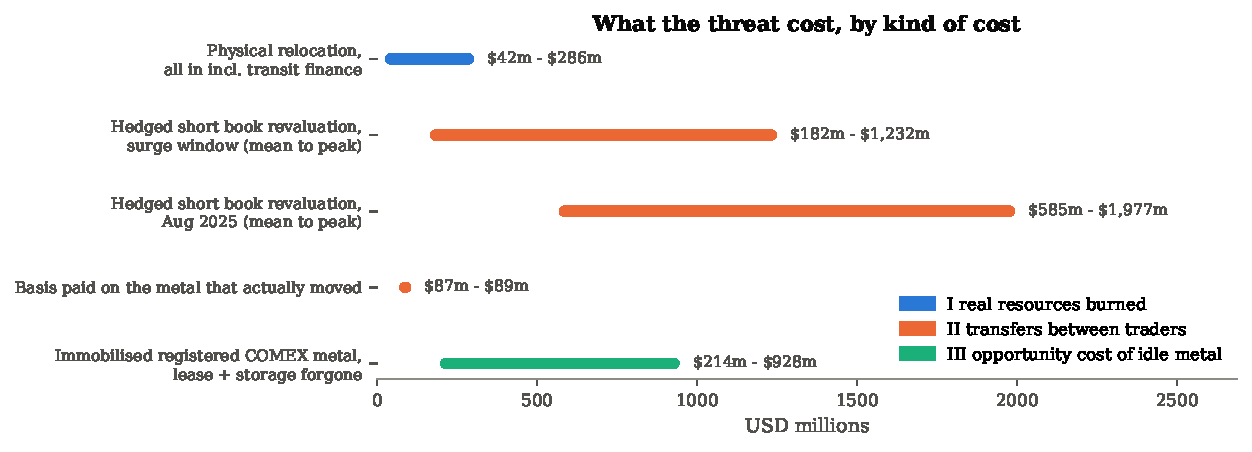
\includegraphics[width=\textwidth]{figures/fig6_ledger.pdf}
\caption{The ledger, by kind of cost.}
\end{figure}

%==============================================================================
\section{What it did to the official numbers}
\label{sec:contamination}
%==============================================================================

\subsection{The reciprocal tariff formula, replicated}

The rates announced on 2 April 2025 were not negotiated. USTR published the formula:
$\Delta\tau_i = (m_i - x_i)/(\varepsilon\,\varphi\,m_i)$ with $\varepsilon = 4$ and
$\varphi = 0.25$, so $\varepsilon\varphi = 1$ and the expression is the bilateral goods deficit
over bilateral goods imports; the announced rate is half of that, floored at 10\%, on calendar
2024 Census data. It replicates exactly.

\begin{center}
\small
\begin{tabular}{@{}lrrrr@{}}
\toprule
\textbf{Partner} & \textbf{2024 imports} & \textbf{2024 exports} & \textbf{Formula} & \textbf{Announced} \\
\midrule
Switzerland & \$63.4bn & \$24.9bn & 30.3\% & 31\% \\
India & \$87.3bn & \$41.6bn & 26.2\% & 26\% \\
China & \$440.3bn & \$143.3bn & 33.7\% & 34\% \\
United Kingdom & \$68.2bn & \$79.5bn & 10.0\% (floor) & 10\% \\
\bottomrule
\end{tabular}
\end{center}

That the formula reproduces four announced rates to the rounding is what makes the
counterfactual below credible: it is the same arithmetic on a different trade base.

\subsection{The intuitive result is wrong in sign}

The natural hypothesis --- and the one this project carried --- is that phantom gold inflated
Switzerland's deficit and therefore its tariff. Removing non-monetary gold from both sides of
the 2024 account gives the opposite:

\begin{center}
\small
\begin{tabular}{@{}lrrrr@{}}
\toprule
& \textbf{Imports} & \textbf{Exports} & \textbf{Deficit} & \textbf{Rate} \\
\midrule
As the formula was run & \$63.4bn & \$24.9bn & \$38.5bn & 30.3\% \\
With gold removed & \$49.4bn & \$15.5bn & \$33.9bn & \textbf{34.3\%} \\
\bottomrule
\end{tabular}
\end{center}

Gold \emph{lowered} Switzerland's computed rate by four percentage points. The reason is that the
corridor is close to balanced in gold --- \$14.0bn in, \$9.4bn out in 2024 --- while the rest of
the relationship (pharmaceuticals, watches, precision machinery) is heavily one-sided. Stripping
gold removes proportionally more from the export side than from the import side and widens the
ratio. This contradicts what the project asserted earlier, and it is the direction the data
gives.

\subsection{The real problem is that the number is a coin flip}

Hold the formula and the country fixed. Vary only which year's data goes in.

\begin{table}[h]
\centering
\small
\begin{tabular}{@{}lrrrr@{}}
\toprule
\textbf{Vintage} & \textbf{US balance} & \textbf{Gold as \% of imports} & \textbf{Rate as run} & \textbf{Rate ex gold} \\
\midrule
2022 & $-\$22.7$bn & 17.2\% & 19.1\% & 33.3\% \\
2023 & $-\$24.5$bn & 13.0\% & 23.4\% & 31.2\% \\
2024 & $-\$38.5$bn & 22.1\% & \textbf{30.3\%} & 34.3\% \\
2025 & $-\$32.5$bn & \textbf{54.3\%} & 15.3\% & 31.8\% \\
2026 (6 mo) & $+\$19.1$bn & 1.9\% & \textbf{10.0\%} (floor) & 27.7\% \\
\midrule
\textbf{Spread} & & & \textbf{20.3 pp} & \textbf{6.6 pp} \\
\bottomrule
\end{tabular}
\caption{Switzerland's reciprocal tariff rate under the published formula, by vintage of trade
data.}
\end{table}

With gold in the data the formula's output for one country ranges over twenty percentage points
across five adjacent vintages. With gold removed the same exercise ranges over six and a half.
Gold makes the instrument \textbf{3.1 times more sensitive} to which year happens to be in the
sample.

Run on 2024 data, Switzerland gets 31\% --- later raised to 39\%. Run on the first half of 2026,
when the same metal was flowing back out and the United States ran a \$19.1bn goods
\emph{surplus} with Switzerland, the identical formula gives the 10\% floor. Nothing about the
Swiss economy changed. The bullion changed direction.

In 2025 non-monetary gold was 54.3\% of everything the United States imported from Switzerland
by value. Of the \$56.0bn of gold the US exported to Switzerland in 2025, \$27.8bn was recorded
as re-exports --- metal that arrived and left again, visible in Census's own re-export line.

\begin{figure}[htbp]
\centering
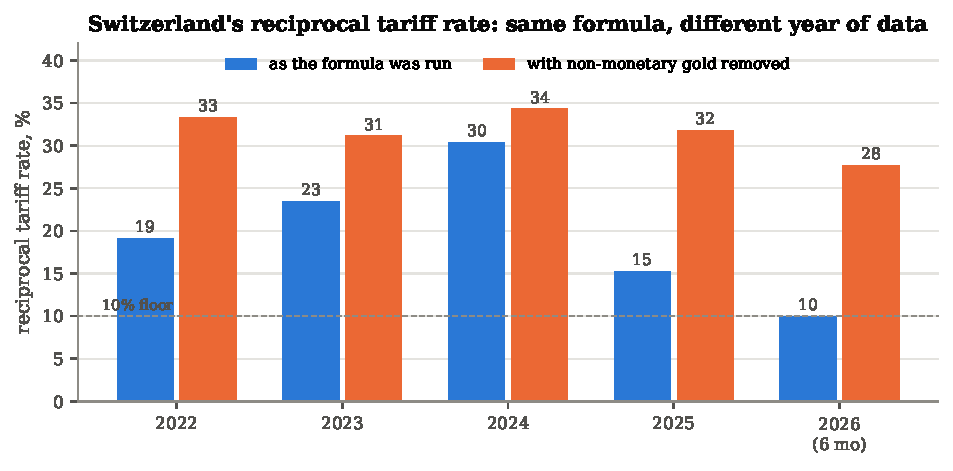
\includegraphics[width=\textwidth]{figures/fig5_tariff_vintage.pdf}
\caption{The same formula, the same country, five adjacent years of data.}
\end{figure}

\subsection{The aggregate trade balance}

The distortion is not confined to one bilateral relationship. Taking the four project partners
only --- so these are lower bounds on total US gold trade:

\begin{center}
\small
\begin{tabular}{@{}lrrr@{}}
\toprule
& \textbf{US goods balance} & \textbf{Net gold imports} & \textbf{Gold as \% of the deficit} \\
\midrule
2025 Q1 & $-\$424.4$bn & $+\$37.0$bn & \textbf{$+8.7\%$} \\
2025 Q4 & $-\$255.7$bn & $-\$29.5$bn & $-11.5\%$ \\
2026 Q1 & $-\$213.5$bn & $-\$33.3$bn & \textbf{$-15.6\%$} \\
\bottomrule
\end{tabular}
\end{center}

In one quarter, metal moving into vaults inflated the measured US goods trade deficit by nearly
nine per cent. Four quarters later, the same metal moving out deflated it by nearly sixteen.
Neither movement corresponded to anything being produced, consumed or invested.

%==============================================================================
\section{What failed}
\label{sec:whatfailed}
%==============================================================================

The project's build order calls for estimating the all-in transatlantic transfer cost from the
kink in the flow--basis relationship, and notes that such an estimate would be publishable on its
own. Two estimators were tried and both failed. Recording that is part of the output.

\subsection{The flow hinge is not identified}

The specification $\text{flow}_t = \alpha + \beta \cdot \overline{\max(0, \text{basis}_d - c)}$,
profiled over a grid of $c$, puts its minimum on the boundary at $c = 0$. This is not evidence
that the transfer cost is zero. Raising $c$ shrinks the regressor close to proportionally, and
the slope absorbs the rescaling, so the sum of squares barely moves: across the entire grid from
\$0 to \$40 an ounce the $R^2$ of the eastbound specification varies by 0.047. The profile is
flat and the argmin carries no information. The project's earlier finding that ``the threshold is
near zero'' is this artefact.

\subsection{The band of inaction is destroyed by the measurement error}

The better estimator is a threshold autoregression on the basis itself: if arbitrage is costly,
the excess basis wanders freely inside a band of half-width $c$ and is pushed back only when it
leaves. Estimated at three sampling frequencies:

\begin{center}
\small
\begin{tabular}{@{}lrrrrr@{}}
\toprule
\textbf{Frequency} & \textbf{$n$} & \textbf{$\hat c$} & \textbf{90\% CI} & \textbf{$\phi$ outside} & \textbf{\% inside} \\
\midrule
Daily & 2,448 & \$0.00 & \$0.00 -- \$60.00 & $-0.76$ & 0\% \\
5-day mean & 489 & \$26.00 & \$12.23 -- \$34.50 & $-1.04$ & 99\% \\
Weekly & 560 & \$0.75 & \$0.50 -- \$49.50 & $-1.06$ & 8\% \\
\bottomrule
\end{tabular}
\end{center}

The three frequencies disagree by an order of magnitude, the confidence intervals span most of
the grid, and the outside-band reversion coefficient sits near $-1$ everywhere. A coefficient of
$-1$ means the series fully reverts in one period: it is white noise around zero, not a price
wandering in a band and being pushed back at its edges. The 5-day fit puts 99\% of observations
\emph{inside} the band and has the inside regime doing the reverting, which is the model
backwards.

The diagnosis is the \S\ref{sec:events} measurement problem. An excess basis built from a
13:30 ET settlement against a 15:00 London auction carries roughly \$16 per ounce of
non-synchronous pricing error per day, and at these frequencies that error is the series.

This does not affect the event study, where the moves being tested are two to four standard
deviations of that same noise and inference is randomization-based against it. It does mean the
transfer cost cannot be read off this series, which is why the ledger uses an assumed range with
sensitivity carried through. Identifying it properly needs a real dealer EFP quote series --- which
lives on entitlement-gated contributor pages --- or intraday-matched London and New York prices.

%==============================================================================
\section{Limitations}
%==============================================================================

\begin{enumerate}[leftmargin=*]
\item \textbf{The unit relocation cost is assumed, not estimated}, for the reasons in
\S\ref{sec:whatfailed}. It is the widest source of uncertainty in Tier I and its range is stated
rather than hidden in a point estimate.

\item \textbf{The gold lease rate is assumed}, over a range spanning a factor of six. Tier III's
range is driven almost entirely by this.

\item \textbf{The COMEX baseline is unobserved.} No archived depository snapshot exists between
20 April 2023 and 30 January 2025. Tier III measures the excess from 30 January 2025, by which
date part of the build had already occurred, so it is a lower bound.

\item \textbf{The hedged short book is an upper bound on London-spread exposure.} The CFTC's
producer/merchant/processor/user and swap-dealer buckets contain more than London-hedged dealer
shorts, and the disaggregated report does not separate them.

\item \textbf{The EFP is a synthetic proxy.} COMEX settlement minus LBMA PM is not a dealer EFP
quote. Episode rankings are robust to this; specific dollar levels are indicative.

\item \textbf{No-interference between Swiss export corridors fails}, quantifiably: 57\% of the
US corridor's rise was offset elsewhere. Both the difference-in-differences and treated-only
estimates are reported for this reason and they bracket a 3\% range.

\item \textbf{The 11 August 2025 event has no published instrument.} It is dated from
contemporaneous reporting of a presidential statement. It is also the largest single-day move in
Table~\ref{tab:events}, so a reader who rejects it should note that the joint test survives
without it.

\item \textbf{The displacement cost is unpriced.} 283 tonnes diverted from consumption markets
is a measured quantity with no price attached, because attaching one requires Indian and Chinese
local premium series this project has not obtained.

\item \textbf{Trade values are nominal.} The gold price rose by roughly two thirds across the
window, so the dollar figures in \S\ref{sec:contamination} mix quantity and price effects. The
tonnage figures do not.
\end{enumerate}

%==============================================================================
\section{Conclusion}
%==============================================================================

A tariff on gold was never imposed and never collected. What happened instead was that for
four months in the winter of 2024--25, and again for a month in the late summer of 2025, market
participants could not be sure it would not be. The first uncertainty was resolvable by moving
metal, and roughly five hundred tonnes moved. The second was not, and the price of location
went to the widest level of the modern era while nothing moved at all.

The resource and opportunity cost of that comes to somewhere between a quarter of a billion and
one and a quarter billion dollars, and the revaluation forced onto hedged short positions
reaches close to two billion at its peak. All of it was spent on a round trip: 1,381 tonnes of
gross bilateral trade for a net position change of minus one and a half tonnes.

Meanwhile the statistical apparatus that trade policy is set from was registering that round
trip as economic activity. The formula that assigned Switzerland a 31\% tariff rate would have
assigned it the 10\% floor on data from eighteen months later, and the difference is not
Switzerland --- it is which way the bullion happened to be pointing when the snapshot was taken.
In one quarter phantom metal inflated the entire US goods trade deficit by nearly nine per cent;
four quarters later the same metal deflated it by nearly sixteen.

The narrow lesson is about gold: bullion is a financial asset that international accounts happen
to record as merchandise, and any policy instrument built on bilateral goods balances will
inherit that error. The broad lesson is about threats. A tariff that is announced and then
withdrawn is not a tariff that did nothing. It is a tariff whose entire cost was paid in
freight, refining, forgone lending and forced revaluation, and none of it collected as revenue.
Uncertainty about a duty is not cheaper than the duty. It is the same cost, spent worse.

%==============================================================================
\section{Reproduction}
%==============================================================================

All scripts are in \texttt{claude/tariff-relocation-cost/code/} and run from the repository root
with \texttt{.venv/Scripts/python.exe}, in numerical order.

\begin{center}
\small
\begin{tabular}{@{}lp{9.4cm}@{}}
\toprule
\textbf{Script} & \textbf{What it does} \\
\midrule
\texttt{01\_events\_and\_us\_che\_trade.py} & Pins the chronology to Federal Register and CBP CROSS documents; parses EO 14346's Annex II flags out of the FR PDF; pulls total US--Switzerland goods trade from Census \\
\texttt{02\_che\_all\_destinations.py} & Re-streams the BAZG bulk zips keeping every partner, for the donor pool. Slow (several minutes per file) \\
\texttt{03\_event\_study\_basis.py} & Event study with randomization inference and the spot-price placebo \\
\texttt{04\_flow\_did.py} & Two-way fixed-effects difference-in-differences, in-space placebos, interference diagnostics \\
\texttt{05\_tariff\_formula\_contamination.py} & Replicates the USTR formula, re-runs it ex gold and by vintage \\
\texttt{06\_transfer\_cost\_kink.py} & The two failed transfer-cost estimators and the bottom-up build \\
\texttt{07\_cost\_ledger.py} & Assembles the ledger; pulls CFTC disaggregated COT \\
\texttt{08\_figures.py} & The seven figures \\
\bottomrule
\end{tabular}
\end{center}

External data pulled live at run time: Federal Register API, Census country trade-balance pages,
CFTC \texttt{publicreporting.cftc.gov}. All are free and unkeyed. Note that
\texttt{api.census.gov} now rejects unkeyed requests, which is why the country balance pages are
used instead; they carry the same published aggregate. FRED was unreachable from this
environment, so no series depends on it.

Everything else comes from \texttt{data/processed/} as built by the existing scripts in
\texttt{src/}. Every number quoted above is written to a JSON file in
\texttt{claude/tariff-relocation-cost/output/} when the scripts are run. That directory is not
committed --- the repository ignores \texttt{output/} under its regenerate-from-source policy ---
so the files appear only after a run.

\end{document}
